\documentclass[a4paper, 10pt]{report}

\renewcommand{\familydefault}{\sfdefault}
\usepackage{amssymb}
\usepackage{mathrsfs}
\usepackage{amsfonts}
\usepackage{amsmath}
\usepackage{graphics}
\usepackage{graphicx}
\usepackage{nomencl}
\usepackage{verbatim}
\usepackage{fullpage}
\usepackage{color}
\usepackage{listings}
\lstset{ %
language=C++,                % choose the language of the code
basicstyle=\footnotesize,       % the size of the fonts that are used for the code
numbers=left,                   % where to put the line-numbers
numberstyle=\footnotesize,      % the size of the fonts that are used for the line-numbers
stepnumber=1,                   % the step between two line-numbers. If it is 1 each line will be numbered
numbersep=5pt,                  % how far the line-numbers are from the code
backgroundcolor=\color{white},  % choose the background color. You must add \usepackage{color}
showspaces=false,               % show spaces adding particular underscores
showstringspaces=false,         % underline spaces within strings
showtabs=false,                 % show tabs within strings adding particular underscores
frame=single,   		% adds a frame around the code
tabsize=2,  		% sets default tabsize to 2 spaces
captionpos=b,   		% sets the caption-position to bottom
breaklines=true,    	% sets automatic line breaking
breakatwhitespace=false,    % sets if automatic breaks should only happen at whitespace
escapeinside={\%}{)}          % if you want to add a comment within your code
}

\title{Notes on Programming}
\author{Robert Simpson}
\date{\today}

\begin{document}
\maketitle

\part{Programming languages}
\chapter{C}

\section{Strings}

We can declare a string in C as follows:

\begin{verbatim}
char string[] = ``Example string'';
\end{verbatim}
Or even allocate an array with more space than is necessary:
\begin{verbatim}
char string[20] = ``Example string'';
\end{verbatim}

The variable ``string'' is basically a pointer to a char so we can make the following assignment
\begin{verbatim}
char* ptr = string;
\end{verbatim}
This feature is used to pass arrays into functions - we pass by reference and not by value. Note that the pointer here is a reference to an existing string, and therefore the string must exist somewhere in memory if are to use it for any sensible reason. 


\section{Variable Types}

There are various variable types that are defined in C, some of which are machine dependent, so be careful!
\begin{table}[htdp]
\caption{default}
\begin{center}
\begin{tabular}{|c|c|}
\hline 
char & single byte\\
int & integer which is implementation defined\\
float & single-precision floating point\\
double & double precision floating point\\
short int & The 'int' can be removed, but this is usually 16 bits long\\
long int & Likewise the 'long' can be removed, but usually 32 bits\\
\hline
\end{tabular}
\end{center}
\label{default}
\end{table}%

In addition, we can have unsigned and signed values for each of the integer types (char, int) which, instead of using the most significant digit to represent the sign of the number, can be used to increase the value of the maximum number. 

To determine the ranges of these variables, we can use the C library functions contained in $<$limits.h$>$. For example:
\begin{verbatim}
#include <stdio.h>
#include <limits.h>

int main(int argc, char* argv[])
{
	printf("The max value of a char is %d\n", CHAR_MAX);
	printf("The min value of a char is %d\n", CHAR_MIN);
	
	printf("The max value of an int is %d\n", INT_MAX);
	printf("The min value of an int is %d\n", INT_MIN);
	
	printf("The max value of an unsigned int is %u\n", UINT_MAX);
	
	printf("The max signed long int value is %ld\n", LONG_MAX);
	printf("The min signed long int value is %ld\n", LONG_MIN);
	
	printf("The max unsigned long int value is %lu\n", ULONG_MAX);
	
	printf("The max signed short int value is %d\n", SHRT_MAX);
	printf("The min signed short int value is %d\n", SHRT_MIN);
	
	printf("The max unsigned short int value is %d\n", USHRT_MAX);
	
	return 0;
}
\end{verbatim}

On my machine, this generates the following output
\begin{verbatim}
The max value of a char is 127
The min value of a char is -128
The max value of an int is 2147483647
The min value of an int is -2147483648
The max value of an unsigned int is 4294967295
The max signed long int value is 9223372036854775807
The min signed long int value is -9223372036854775808
The max unsigned long int value is 18446744073709551615
The max signed short int value is 32767
The min signed short int value is -32768
The max unsigned short int value is 65535
\end{verbatim}



\section{Octal and Hexadecimal}

To represent a number in octal, we precede the number with a zero. Therefore the number 
\begin{verbatim}
0177
\end{verbatim}
represents 127 in base 10 notation. To represent a hexadecimal number, we precede the digits with 0x:
\begin{verbatim}
0x11
\end{verbatim}
which represents 17 in base 10.

\section{Enumeration}

To generate a list of constant values which represent certain values, it is often convenient to use enumerated lists. These can be generated like:
\begin{verbatim}
enum boolean {no, yes};
\end{verbatim}
Or with certain values specified:
\begin{verbatim}
enum escapes {BELL = '\a', BACKSPACE = '\b', TAB= '\t'};
\end{verbatim}

\section{Condition expressions}

A really nice an succint way of writing an if ... else ...statement is by
\begin{verbatim}
z = (a > b) ? a : b;
\end{verbatim}
Which basically defines a function z=max(a,b). It is equivalent to 
\begin{verbatim}
if (a > b)
	z = a;
else 
	z = b;
\end{verbatim}

\section{Functions}

\subsection{Inline functions}

If you see the keyword ``inline'' at the beginning of a function then this tells the compiler than whenever this function is called, then the entire function is replaced by the call in the machine code. It should only be used for small functions and should theoretically speed up the code. However, the compiler may choose to ignore the inline function.


\section{Small Hints}

\subsection{Why do we use int instead of char for getchar()}
This is detailed on pg. 16 of K \& R, but the reason comes down to one simple fact. If we use a char to represent character input this is fine if the only input is any real character (eg. 'a', 'A', '0' ...). But if we want to terminate the input with the EOF character, then we need a variable which is capable of holding not only every possible real character, but also the EOF character. The variable char is not big enough to do this, so we use int as a compromise.  

\subsection{Increment and decrement operators}

We can use the following increment operators
\begin{verbatim}
++ 	: 	increment (add one)
--	: 	decrement (subtract one)
\end{verbatim}
But there is subtle different if we use these operators as a suffix or a prefix. Consider the following:
\begin{verbatim}
n = 5;
x = n++;
\end{verbatim}
Here, x will equal 5. Now consider
\begin{verbatim}
n = 5;
x = ++n;
\end{verbatim}
x will now equal 6. Using the operator as a prefix means that the increment operator is applied before the variable is used. This can be useful in many scenarios.

\subsection{EOF}

On the mac, the End Of File character is given by Ctrl-D. So we may get input in a C program using 
\begin{verbatim}
int c;
while((c = getchar()) != EOF) {
 ...
}
\end{verbatim}

\section{Standard Library}

\subsection{Ctype.h}

\subsection{isspace(int)}

This function determines whether or not the character being passed in is a white-space character (eg newline, tab, space, carriage-return). and will return a non-zero value if so. eg.
\begin{verbatim}
#include <stdio.h>
#include <ctype.h>

int main(int argc, char* argv[])
{ 
    char* string = "This is the string to test for \n characters etc.\t\t";
    printf("%s\n", string);

    int c = 0;
    while ( string[c] != '\0' ) { 
        printf("%d", isspace(string[c]));
        c++;
    }   

    return 0;
}
\end{verbatim}
This outputs:
\begin{verbatim}
This is the string to test for 
 characters etc.		
00001001000100000010010000100011100000000001000011
\end{verbatim}




\chapter{C++}

\section{Classes}

\subsection{Constructors}

\subsubsection{Explicit constructors}

\emph{BS: \S11.7.1}

We find that by default, constructors without any ``explicit'' keyword are converting constructors. For example, if we take a simple class with several constructors:
\begin{verbatim}
class MyClass {
	MyClass();
	MyClass(int);
	MyClass(const char*, int);
};
\end{verbatim}
we can create objects using an implicit conversion as:
\begin{verbatim}
MyClass a = 5;
MyClass b = ``booya!'';
\end{verbatim}
where the first line is equivalent to 
\begin{verbatim}
MyClass a = MyClass(5);
\end{verbatim}

If we now prefix each of the constructors with the keyword ``explicit'', then the previous lines of code would be illegal. 
\begin{verbatim}
class MyClass {
	explicit MyClass();
	explicit MyClass(int);
	explicit MyClass(const char*, int);
};
\end{verbatim}
and we would need to call constructors as follows:
\begin{verbatim}
MyClass a = MyClass(5);
MyClass b = MyClass(``booya!'');
\end{verbatim}


\subsubsection{Default arguments}

\emph{BS: pp. 226-228}

Sometimes it might be useful for a constructor to take on default values. Take for example, the following class definition:
\begin{lstlisting}
class Date {
	int d, m, y;
	public:
		Date(int dd = 0; int mm = 0; int yy = 0);
};
\end{lstlisting}
with the following implementation
\begin{verbatim}
Date::Date(int dd, int mm, int yy)
{
	d = dd;
	m = mm;
	y = yy;
}
\end{verbatim}
We can call this in the following ways
\begin{verbatim}
Date date();
Date date2(2,3,2012);
Date date3(4,5);
Date date4(5);
\end{verbatim}

We can also shorten the code of the constructor by defining it using an \emph{initialiser list} as follows:
\begin{verbatim}
class Date {
	int d, m, y;
	public:
		Date(int dd = 0, int mm = 0, int yy = 0) : d(dd), m(mm), y(yy);
};
\end{verbatim}

It is also possible to specify optional arguments for a function (not just a constructor) in the following manner
\begin{lstlisting}
void function(int arg, int option = 0)
{
 /* Some code */
}

function(int c = 5);
function(int c = 5, int d = 6);
\end{lstlisting}
In the first case we would find that the function would set option = 0. It should also be noted that the default arguments must come at the \emph{end} of the argument list.

\subsection{Copy constructors}

The purpose of a copy constructor is to allow code like the following to be written
\begin{lstlisting}
Date B = Date(2,3,2012);
Date A = Date(B); 	/* We have created an object from another */
\end{lstlisting}
So we can imagine a copy constructor looking like a normal constructor except that it takes an object as an argument. It looks like the following
\begin{lstlisting}
/* Date.cpp */

Date::Date(const Date& rhs)
{
	d = rhs.d;		/* This might seem bizarre that we are using private members of 'rhs' */
	m = rhs.m;
	y = rhs.y;
}
\end{lstlisting}
What is slightly baffling is that we are using private members of the passed in reference to initialise the present object. What we must realise is that \emph{access specifiers act on a class level and not an object level}. Therefore, since we are in a member function of Date, and the passed in argument ('rhs') is of type Date, then we can access the private members of 'rhs' within this function. 

Astute readers may notice that the copy constructor above is not the only function we require, since the assignment operator '=' is also required. We usually write the assignment operator as follows, making sure to check for self-assignment
\begin{lstlisting}
Date& Date::operator= (const Date& rhs)
{
	if ( &rhs == this ) return *this;		/* Check for self-assignment */
	
	d = rhs.d;
	m = rhs,m;
	y = rhs.y;
	
	return *this;
}
\end{lstlisting}


\subsection{Destructors}

\subsubsection{The importance of virtual destructors}

The idea of virtual functions is that the correct function is called according to the type of object created. In many cases we may wish to decide what type of object to create at runtime, like in the following example.


Here we have created a pointer to a base class of type Base. Depending on the value of i, we either create an object of type Derived or type Base. This can only be determined during runtime. Once we are finished with the object, we delete it. At this point an appropriate desctructor must be called which brings us onto the subject of virtual destructors. If the pointer b is of type Derived, then we must ensure that not only the Derived class desctructor is called, but also the Base class destructor. This can be achieved in the following way
\begin{lstlisting}
class Base {
public:
   Base() { cout << "Constructor called" << endl; }
   virtual void sayHello() { cout << "Hi from Base" << endl; }
    virtual ~Base() { cout << "Desctructor from Base called" << endl; }
};

class Derived : public Base {
public:
     Derived() {cout << "Derived constructor called" << endl; }
     void sayHello() { cout << "Dervied says hello" << endl;}
     ~Derived() { cout << "Dervied destructor called" << endl; }
};
\end{lstlisting}
If we left out the keyword virtual, then if a Derived object is created the correct destructor will never be called. Instead, since the pointer is of type Base*, only the Base destructor will be called. This could create mayhem if these classes used dynamic memory.

\subsection{Assignment operator}

C++ creates a default assignment operator (if none is prescribed) which will simply copy all the members of one object to another \emph{by value}. This is fine until we have dynamic memory and pointers presribed in our class definition, and we get some nasty bugs. Frequently, the default mechanism for copying is referred to as ``shallow'' copying which means that we copy the member variables using the default assignment mechanics. But if this mechanism was applied to a pointer which pointed to dynamically allocated memory, then we would simply copy the address of the pointer which would lead to some nasty results (such as deleting memory twice). Instead, we wish to perform a ``deep'' copy, where we copy the object being \emph{pointed to}, not the pointer itself.

We can imagine an arbitrary class where with as assignment operator as follows:
\begin{lstlisting}
class Base {
	int x;
public:
	Base(int initVal = 0) : x(initVal) {};
	Base& operator=(Base& rhs);
};

Base& Base::operator=(Base& rhs)
{
	if ( rhs == &rhs ) return *this;
	
	x = rhs.x;
	return *this;
} 

int main()
{
	Base b = Base(0);
	Base c = Base(2);
	
	b = c;	//	b is assigned x = 2
	
	return 0;
}
\end{lstlisting}

But we may end up with a problem when we used a derived class. Imagined a class which is dervied from Base in the following way:
\begin{lstlisting}
class Derived : Base 
	int y;
public:
	Derived(int intVal) : Base(initVal), y(initVal) {};
	Derived& operator=(Derived& rhs);
};

Derived& Derived::operator=(Derived& rhs)
{
	if (this == &rhs) return *this;
	
	y = rhs.y;
	return *this;
}
\end{lstlisting}
The problem with this is that if we perform an assignment on the derived class then we will not copy across the members belonging to the base class (ie. x will not be assigned in this case). To solve this, we must make a call to the base class assignment operator in the following way
\begin{lstlisting}
Derived& Derived::operator=(Derived& rhs) 
{
	if (this == &rhs) return *this;
	
	Base::operator=(rhs);		//	 this calls the base class assignment operator
	y = rhs.y;
	return *this;
}	
\end{lstlisting}
Job done!

\subsection{Static members}

\emph{BS: pp. 228-229}

Sometimes we might wish to have a variable that is common amongst objects of the same type. This is where static members come in handy. The idea is that there will exist only one instantiation of static members, rather like a 'global' variable. In addition, we can create static member functions which do not have any 'this' pointer. Therefore it is meaningless to access member data through a static function. Let's consider a static member and a static function.
\begin{lstlisting}[label=static,caption=Static members]
class Date
{
	static Date default_date;
	int d, m, y;
	
	public:
		Date(int dd=0, int mm=0, int yy=0);	// constructor with default arguments
		
		static void setDefault(int dd, int mm, int yy);
};

Date Date::default_date(23,2,2012);	// IMPORTANT: we must create it in memory

void Date::setDefault(int dd, int mm, int yy)
{
	default_date = Date(dd,mm,yy);
}

int main(int argc, char* argv[])
{
	Date::setDefault(5,12,2012);
	return 0;
}
\end{lstlisting}
Notice that we must create an instance of the static member, otherwise it will not exist in memory. We can refer anywhere to the function 'setDefault' by including the scope operator :: . 

\subsection{Return values from functions}

We must ensure that we do not return pointers or references to local variables defined in functions since otherwise, when the function goes out of scope (ie all local variables disappear in memory), the pointer or reference will contain garbage. Fortunatley most compilers will catch this sort of error.

An interesting example which demonstrates an example of where we can return a reference (ie. an alias of a variable) in a chained manner is follows:
\begin{lstlisting}[label=chained,caption=Chained operations]
class Date {
	int d, m, y;
pubic:
	Date(int dd=0, int mm=0, int yy=0);
	Date& addDay(int dd);
	Date& addMonth(int mm);
	Date& addYear(int yy);
};

Date::Date(int dd, int mm, int yy)
{
	d = dd; m = mm; y = yy;
}

Date& Date::addDay(int dd)
{
	d++;
	return *this;	//	ok to return dereferenced this, since it exists outside this scope
}

Date& Date::addMont(int mm)
{
	m++;
	return *this;
}

Date& Date::addYear(int yy)
{
	y++;
	return *this;
}

int main()
{
	Date someDate(23,2,2011);					//	create a date
	someDate.addDay(1).addMonth(1).addYear(1);	//	notice the chained operations
	return 0;
}
	
	
\end{lstlisting}


\subsection{Inline member functions}

Inline functions are a flag for compilers which give them the option to apply optmisation to the function. If a function is simple, then the compiler can usually replace any call to the relavant function with the code of the function rather than a call to the function. We therefore only apply inline to functions which are simple in nature. Remember though, that inlining is applied at the compiler's discretion. 

One feature which should be mentioned is the automatic inlining of member functions which are defined in the class declaration. For example:
\begin{lstlisting}
class Dave {
	int weight;
pubic:
int getWeight() { return weight; }
/* other public functions */
};
\end{lstlisting}
The public member function ``getWeight()'' is automatically an inline function since it is included in the class declaration (Str. p. 235)

\subsection{Overloaded operators}
There are several operators that can be overloaded in C++ to create nice user interfaces for classes. Some of the most common overloaded operators include:
\begin{lstlisting}
operator()
operator=()
operator+=()
operator+()
operator*()
\end{lstlisting}
Such functions are extremely useful for defining types such as matrices and vectors, since operations like \verb#v(4) = 5#, \verb#M(4,5) = 5#  are possible. Let's assume that we are trying to declare functions that would perform such operations on a vector class. We would in fact need two definitions given by:
\begin{lstlisting}
inline double& Vector::operator(const int i) { return A[i-1]; }
inline double Vector::operator(const int i) const { return A[i-1];} 
\end{lstlisting}
The reason we have two is because we want to use the operator for both const and non-const vector objects, otherwise it would be perfectly feasible to use the first definition. We have also used the inline keyword which tells the compiler we wish to replace all calls to his function with the definition of the function (rather than a call to the function), which implies that these two lines will be written in the declaration of the class and will be located in a header file.

\subsubsection{Friend functions and classes}

There is a feature in C++ that allows a function to access the private members of classes, even if the function itself is not a member function of those classes. For example, imagine two classes like so:
\begin{lstlisting}
class Man {
double weight;
int numCansBeerDrunk;
public:
	Dave() : weight(0.0), numCansBeerDrunk(0) {}
	Dave(double w, int numCans) : weight(w), numCansBeerDrunk(numCans) {}
	getWeight() { return weight; }
	getNumCansDrunk() { return numCansBeerDrunk;} 
};

class Woman {
double weight;
int numGlassesWineDrunk;
public:
	Woman() : weight(0.0), numGlassesWineDrunk(0) {}
	Woman(double w, int numGlasses) : weight(w), numGlassesWineDrunk(numGlasses) {}
	getWeight() { return weight;}
	getNumGlassesDrunk() { return numGlassesWineDrunk; }
};
\end{lstlisting}

And say we define a function that calculates the total number of units of alcohol that a couple drink:
\begin{lstlisting}
int totalAlcoholUnitsForCouple( Man& man, Woman& woman)
{
	return man.numCansBeerDrunk + woman.numGlassesWineDrunk;
}
\end{lstlisting}
It should be stressed that because this function tries to access the private members of the classes Man and Woman, this will fail to compile. To allow the function access to private members, we declare the funciton as a \emph{friend} function of each class like so:
\begin{lstlisting}
class Woman;

class Man {
/* private members */
public:
	/* public members */
	friend int totalAloholUnitsForCouple(Man& man, Woman& woman);
};

class Woman {
/* private members */
public:
	/* public members */
	friend int totalAloholUnitsForCouple(Man& man, Woman& woman);
};
\end{lstlisting}
Now the code will compile, and the function has full access to the private members of both classes. Notice also that a forward declaration of the Woman is required since the class Man knows nothing about the Woman class yet it declares a function with a Woman argument.


\section{Class design}
\label{sec:class-design}

\subsection{Composition}
\label{sec:composition}

\subsection{Aggregation}
\label{sec:aggregation}

A way of creating classes that are made up on references
(ie. pointers) to other classes is known as aggregation. The key idea
is that within the class there are member variables which are
pointers to the objects that exists outside the class. In contrast to
composition, where the objects exists inside the class (and therefore
will cease to exist when the class is destroyed), the class does not
own the objects directly and they will continue to exist once the
class is destroyed. 

Consider an example of a Duck class defined as follows:
\begin{lstlisting}
// Creation of a "Duck" class
#include <iostream>

class Duck
{
	private:
	
	bool isflying;
	double speed;
	double coordx,coordy,coordz;

	public:

	Duck( double x = 0.0, double y = 0.0, double z = 0.0, double s = 0.0 ) :
	coordx(x), coordy(y), coordz(z), speed(s), isflying( s > 0.0 )
	{
	}

	~Duck()
	{
	}

	friend std::ostream& operator<<(std::ostream& out, const Duck& duck)
	{
		std::cout << "Duck flying? " << duck.isflying << "\n";
		std::cout << "speed = " << duck.speed << "\n";
		std::cout << "x = " << duck.coordx << "\n";
		std::cout << "y = " << duck.coordy << "\n";
		std::cout << "z = " << duck.coordz << "\n";

		return out;
	}
	
};
\end{lstlisting}
We wish to create a Pond class which hold several ducks. If this were
to be designed using composition, we could create such a class by
defining, say, a list of ducks as 
\begin{verbatim}
std::list<Duck> mlistofducks;
\end{verbatim}
and we could possibly design the class in such a way that we create
copies of the ducks that exist outside the Pond class. As soon as we
create copies, then the Ducks that exist inside the pond class are
in no way related to those outside. This might be fine for our
purposes, but if we have very large Ducks (not physically, but the
size of their classes), then this will be very inefficient. 

Instead, we store pointers to the required Ducks and store those
pointers within a list like so:
\begin{verbatim}
std::list<Duck*> mlistofducks;
\end{verbatim}
Note that this is list of pointers. In this manner we could create a
Pond class like so:
\begin{lstlisting}
#include <iostream>
#include <list>

class Duck;

class Pond
{
	private:

	std::list<Duck*> mducksInPond;

	double mtemperature;

	public:

	Pond( double t = 0.0, std::list<Duck*> ducks = std::list<Duck*>() ):
	mtemperature(t), mducksInPond(ducks)
	{}

	~Pond()
	{

	}

	void addDuck( Duck* duck )
	{
		mducksInPond.push_back(duck);
	}

	void printSizes()
	{
		std::cout << "Pond temp = " << mtemperature << "\n";

		std::cout << "num ducks = " << mducksInPond.size() << "\n";
	}
	

	friend std::ostream& operator<<(std::ostream& out, const Pond& pond)
	{
		std::cout << "Pond temperature = " << pond.mtemperature << "\n";

		Duck* present_duck;
		
		for( std::list<Duck*>::const_iterator it = pond.mducksInPond.begin(); it != pond.mducksInPond.end(); it++)
		{
			std::cout << *(*it) << std::endl;
		}
		return out;
		
	}
	
};
\end{lstlisting}
In this class we initialise the Pond with a double and list of
pointers to ducks. In addition, we can add a duck to our list through
the member function addDuck(). We could use this class like so:
\begin{lstlisting}
#include <iostream>
#include <list>
#include "Duck.h"
#include "Pond.h"

int main()
{
	// A simple aggregate example where we create some ducks and pass their references
	// to a pond class. So the pond doesn't actually own the ducks, but it can access
	// the informaion through their pointers.

	// creat a duck
	Duck myduck(5,5,5,5);
	std::cout << myduck << std::endl;

	// create another duck
	Duck anotherduck(2,3,4,5);
	std::cout << anotherduck << std::endl;

	// create a list of pointers to ducks
	std::list<Duck*> listofducks;
	// add the ducks pointers to the list
	listofducks.push_back(&myduck);
	listofducks.push_back(&anotherduck);

	// create a point with the list of pointers of ducks as an argument
		{
			
			Pond littlepond( 5.0, listofducks);
			std::cout << littlepond << std::endl;

			// now create a null duck and add to the pond
			Duck duckthree;
			littlepond.addDuck(&duckthree);
	
			std::cout << littlepond << std::endl;
		}

		// the pond has gone, so let's check our ducks exist
		std::cout << myduck << std::endl;

		return 0;
}
\end{lstlisting}

\subsection{Inheritance}

This is a subject that often confuses me, and sometimes I find it difficult know what level of access certain members of a class should be given. From talking to experience programmers, it seems that these things will make more sense as you program more. But perhaps the C++ syntax which I find most confusing is 'protected' inheritance. I understand that private members are only visible to the class itself and cannot be use in subclasses and that public members can be used by anyone, but protected is slightly difference. It can be used only \emph{derived} classes.  But why would we want to use it? Let's have a look at an example. Consider a class called Vehicle which is intended to be an abstract class. A definition might look like follows:
\begin{lstlisting}
class vehicle
{
private:

int numberPassengers;
double speed;

protected:
Vehicle();
virtual void systemsCheck();

public:
virtual void accelerate() = 0;
virtual void brake() = 0;
void addPassenger();
void removePassenger();
int getPassengerNum();
double getSpeed();
~virtual Vehicle();
};
\end{lstlisting}
Here we know this vehicle class is abstract due to the use of pure virtual functions, and therefore this class will never be instantiated. The member variables numberPassengers and speed are private and cannot be accessed by any derived classes. But the protected members require a bit extra thought. These can be accessed by derived classes but nowhere else. We have put the constructor here because we never instantiate this class, but the constructor will be used in the initialisation list of dervied classes. 





\section{Memory management}
\label{sec:memory-management}

Whenever we deal with objects that are created on the ``heap''
(ie. through dynamic allocation), then we must be very careful about
how we manage our memory through such objects. Fortunately, there
exists a number of specially written classes which can help us manage
dynamic memory in a robust way. Two such objects are: auto\_ptr and tr1::shared\_ptr

\subsection{auto\_ptr}
\label{sec:auto_ptr}

The autoptr class allows us to create objects on the heap and not
worry about cleaning them up afterwards. The way that his works is
that when the object goes out of scope, the destructor for the object
is called and the memory is released. We may create an auto\_ptr as
follows:
\begin{lstlisting}
#include<memory>
#include<iostream>

int main()
{
	std::auto_ptr<int> pint(new int);
	std::cout << ''Address of pint is '' << pint.get() << std::endl;
	
	// Use copy constructor to create a copy of pint
	std::auto_ptr<int> pint2(pint);
	std::cout << ''Address of pint2 is '' << pint2.get() << std::endl;
	std::cout << ''Address of pint is '' << pint.get() << std::endl;
	return 0;
} 
\end{lstlisting}
The first thing to notice that there is no call to delete[] since we
are using an auto\_ptr - the memory resources are handled
automatically. But this example also illustrates the shortcoming of
auto\_ptr - that when we copy an auto\_ptr, we pass ownership of the
resource onto the newly created pointer. The original pointer then has
a nil pointer which points to nothing. Therefore, we should be very
careful when copying auto\_ptrs since we may not get the behaviour we
expect.

\subsection{tr1::shared\_ptr}
\label{sec:tr1::shared_ptr}

To overcome the limitations of auto\_ptrs, we can use a
tr1::shared\_ptr which gives more natural behaviours. It implements a
reference counting mechanism whereby the number of pointers that are
referring to the objects is kept track of. Then, when this number
reaches zero, we know that nothing is pointing to the object and the
appropriate memory can be released. 

The following code demonstrate the use of the tr1::shared\_ptr along
with a comparison with the auto\_ptr.
\begin{lstlisting}
#include <iostream>
#include <memory>
#include <tr1/memory>

// Demonstrating the use of smart pointers in C++

// We show both auto_ptr and tr1::shared_ptr (which is more flexibile and uses
// a reference counting mechanism)

class dummy
{
	public:
	void print()
		{
			std::cout << "Address of this dummy = " << this << std::endl;
		}
	~dummy()
		{
			std::cout << "dummy desctructor called" << std::endl;
		}
	
};

int main()
{
	// create an auto ptr which refers to a dummy
	{
		std::auto_ptr<dummy> p1(new dummy);
		p1->print();
		
		// and now create a copy of p1 (default behvaviour is to pass ownership
		std::auto_ptr<dummy> p2(p1);
		p1->print();
		p2->print();
	}
	

	std::cout << "Now the tr1 pointers" << std::endl;
	
	// now try the same with tr1::shared_ptr
	std::tr1::shared_ptr<dummy> pt1(new dummy);
	pt1->print();

	std::tr1::shared_ptr<dummy> pt2(pt1);
	pt1->print();
	pt2->print();
	
	std::cout << "Reference count of pt1 = " << pt1.use_count() << std::endl;
	std::cout << "Reference count of pt2 = " << pt2.use_count() << std::endl;
	
	return 0;
}  
\end{lstlisting}

\subsubsection{Use with std containers}
\label{sec:use-with-std}

We can also use the tr1::shared\_ptr with the std containers. Here is
an example code which shows its use with containers.

\begin{lstlisting}
#include <iostream>
#include <tr1/memory>
#include <vector>
#include <algorithm>

// the idea of this program is to show that tr1::shared_ptr can be used with the
// std containers

// function to double the value pointed to by a shared_ptr
std::tr1::shared_ptr<int> double_value(const std::tr1::shared_ptr<int>& in)
{
	*in *= 2;
	return in;
}

int main()
{
	// first create the vector of tr1_shared_ptrs
	std::vector<std::tr1::shared_ptr<int> > vecpints;
	// create a shared ptr
	std::tr1::shared_ptr<int> pint(new int(5));
	// add shared ptrs to the vector
	vecpints.push_back(std::tr1::shared_ptr<int>(new int(1)));
	vecpints.push_back(std::tr1::shared_ptr<int>(new int(2)));
	vecpints.push_back(std::tr1::shared_ptr<int>(new int(3)));
	vecpints.push_back(pint);
	vecpints.push_back(pint);

	// output the array
	for(std::vector<std::tr1::shared_ptr<int> >::iterator it = vecpints.begin();
		it != vecpints.end();
		++it)
		std::cout <<  *(*it) << " and reference count = " <<  (*it).use_count() << std::endl;

	// now perform a groovy little "transform" on the vector
	std::transform( vecpints.begin(), vecpints.end(), vecpints.begin(), double_value);
	for(std::vector<std::tr1::shared_ptr<int> >::iterator it = vecpints.begin();
		it != vecpints.end();
		++it)
		std::cout <<  *(*it) << " and reference count = " <<  (*it).use_count() << std::endl;
	
	return 0;
}

\end{lstlisting}

\subsubsection{General usage of smart pointers}
\label{sec:general-usuage-smart}

One thing which bothers me is deciding when to use smart pointers. For
instance, in some of the classes I use for my numerical analysis I
need to refer to a particular ``Mesh'' object to get information about
the geometry of the model. Now should I implement this as a
shared\_ptr where every other class that refers to it increases the
reference count?

Well I did a bit of background research on the subject and I think I
am come to the following conclusion: reference counting is only
relevant for cases when we have \textit{multiple objects owning the
  same object.} What I have in my example for the Mesh object is a
``has-a'' relationship where the objects simply refer to the Mesh and
do not own in. This is expressed as  (in computer science
speak) aggregation.

But what smart pointers are designed for is dealing with memory
management issues. So what might be a good design is to create the
Mesh object as a smart pointer and then to assign this to each
of the objects that use this Mesh by storing it as a raw pointer.


\section{Header and source files}

Conventionally we use the extension {\bf .h} for header files and {\bf .cpp} for source files. Some important points
\begin{itemize}
\item Generally the header files contain function prototypes, preprocessor directives and type definitions
\item The source files contain the function definitions
\item We must {\bf \#include} any header files in the source files if we need them. 
\item When we compile a program we just use the {\bf .cpp} files 
\end{itemize}

When we compile a program what we end up with is a an object file (which is also referred to as the binary). It usually has the extension {\bf .obj}. Then, by performing appropriate linkage, the object file can then be converted to an executable which can be used by the user.

One term which is commonly used is the term \emph{translation unit}. This refers to a source file which its associated header files that need to be included.   

\section{Templates}

In the case that we want to generate several version of a class or function where only the type of a certain variable changes in each instant, it is preferable to use templates rather than create separate versions. It should be noted though, that the code we write using templates may be shorter in length but in fact the compiled code would be just as long as if the individual versions of the code were written in full. 

\subsection{Function templates}

The best way to illustrate the use of templates is to give a example. 

\begin{verbatim}
template <class T> T max(T x[], int length) 
{
	T max = x[0];
	for(int i=1; i< len; i++)
		if(max<x[i])
		  max=x[i];
	return max;
}
\end{verbatim}
As can be seen, the only difference is the use of \emph{template <class T>} compared to a normal function definition. Also, if we were to replace every instance of \emph{T} with, say, \emph{double}, then we can see that we would end up with a function where the array \emph{x} is defined as a double and the value returned is also a double. 

If we wished to use this function where \emph{T} is defined as a double, we would write the template definition first (or include it if it is in a different file) and then we might write the following
\begin{verbatim}
int main(void)
{
double large[] = {0.0, 1.0, 2.0, 3.0, 4.0, 5.0, 6.0};
int lenLarge = sizeof large/ sizeof large[0];
double maxValue = max(large, lenLarge);

return 0;
}
\end{verbatim}

\subsection{Class templates}

Class templates are something which really takes a while to get your
head around. We can imagine a class template as a kind of ``factory''
which is able to produce many different objects. The best way to
understand how templates are used is to play around with standard
library classes such as vector, map, list etc. since these use class
templates heavily. 

But let's say that we want to produce our own class template, so we
want to know what the syntax is like. Imagine a vector class that we
want to instantiate in such a way that we could create a vector of
ints or a vector of doubles. We could imagine creating such vectors
like
\begin{verbatim}
vector<int> intVector;
vector<double> doubleVector;
\end{verbatim}
We see that the type is passed in as an argument using the angle
brackets - you will see these brackets many times when you work with
templates!

Now let's consider a template class definition, which might be written
like 
\begin{lstlisting}
template<class T>
class vector
{
private:
	T* data;
	int sz;

public:
	vector(const int size) : sz(size), data(new T[size]) {}
	~vector() { delete[] data; }

	inline T& operator(const int i) 
	{
		return data[i];
	}
	inline int size() { return sz; }
};
\end{lstlisting}



Taken from pp. 73-80 of the ``Diffpack'' book.

A few points that I have picked up:

\section{Include guards}

To avoid multiple inclusion of header files, it is necessary to use header guards that are standard in c++ code. They have the following form 
\begin{verbatim}
#ifndef OURHEADERFILE_H_IS_INCLUDED
#define OURHEADERFILE_H_IS_INCLUDED

// .. and our code goes in here for our header file

#endif
\end{verbatim}

What happens here is that when we include this header file within a .cpp file the macro OURHEADERFILE$\_$H$\_$IS$\_$INCLUDED is defined. Then, if we try to include the same file again within the .cpp file we see that it is already included - nothing more needs to be done. This will avoid any compilation errors in our code when including the header file twice. 

\begin{itemize}
\item We can make use of inline functions which basically mean that the compiler will replace any calls to the function by the code of the function itself. This will speed up any code that calls the function many times. In particular, we may wish to do this for the $()$ operator function that is used to access elements of a vector.
\item We should make use of the \emph{const} keyword as much as possible. Functions too can also be const by putting the keyword at the end of the function description. This will then mean that the function will not alter the pointer \emph{this} and it is safe to use this functions on constant objects. Otherwise, we could end up with a function altering an object we have defined as constant. 
\end{itemize}


\section{Inheritance}

\subsection{Access specifiers}

When a class is derived from another [base] class, we have the option to put in an \emph{access specifier} which determines how the members of the dervived class can access the base class members. If we do not specify anything, then by default the access specifier is \emph{private}. There are three dfferent scenarios we may encounter, the most common of which is the public access specifier. Let's consider what happens:

\begin{lstlisting}
class A {
	int priv_A;
protected:
	int prot_A;
public:
	int pub_A;
};

class B : public A {
	int priv_B;
protected:
	int prot_B;
public:
	int pub_B;
};

int main()
{
	A testA;
	test.pub_A = 1;
	B testB;
	testB.pub_A = 1; 	// we can still access this member - it is inherited as public
	testB.prot_A = 1;	// error since this member is inherited as protected
	testB.priv_A = 1;	// error since this member is inherited as private
	return 0;
}	
\end{lstlisting}
The general idea of public inheritance is that the members of the base class and inherited keeping their original specifiers. So a public member will remain public, protected remains protected and private is still private.

The protected access specifier is one that is used rarely and can be a bit of struggle to get your head around. The way I look at it is to imagine a filter being applied when we derive a class using an access specifier. Any member which has a level of access above that of the access specifier is `chopped' down to agree with the access level. So in this way, if we were to use `protected', then public members would become protected, protected members would become protected and private would remain private. eg. 

\begin{lstlisting}
class A {
	int priv_A;
protected:
	int prot_A;
public:
	int pub_A;
};

class B : protected A {
	int priv_B;
protected:
	int prot_B;
public:
	int pub_B;
	B() 
	{
		priv_A = 1; 	// error - this is private to A
		prot_A = 1; 	// fine - this is protected in B
		public_A = 1; 	// fine - this is protected in B
	}
};

int main()
{
	A testA;
	test.pub_A = 1;
	B testB;
	testB.pub_A = 1; 	// error - this is now protected
	testB.prot_A = 1;	// error since this member is inherited as protected
	testB.priv_A = 1;	// error since this member is inherited as private
	return 0;
}	
\end{lstlisting}

And finally we have private access, which means that all members in the derived class become private. 
\begin{lstlisting}
class A {
	int priv_A;
protected:
	int prot_A;
public:
	int pub_A;
};

class B : protected A {
	int priv_B;
protected:
	int prot_B;
public:
	int pub_B;
	B() 
	{
		priv_A = 1; 	// error - this is private to A
		prot_A = 1; 	// fine - this is private in B
		public_A = 1; 	// fine - this is private in B
	}
};

int main()
{
	A testA;
	test.pub_A = 1;
	B testB;
	testB.pub_A = 1; 	// error - this is now private
	testB.prot_A = 1;	// error since this member is inherited as private
	testB.priv_A = 1;	// error since this member is inherited as private
	return 0;
}	
\end{lstlisting}

\subsection{Copy constructors and assignment operators in derived classes}
\label{sec:copy-constr-assignm}

In most cases we can simply use the default copy constructor and
assignment operator as created by the compiler, but when we explicitly
declare them ourselves, we must take extra care when dealing with
classes that are derived from others. Scott Meyers gives an excellent
explanation of this in his book ``Effective C++'' in the section
entitled ``Copy all parts of an object''.

Let's explain the scenario through an example.

Consider a base class in which we define a custom copy constructor and
assignment operator:
\begin{lstlisting}
class Base
{
     public:
      
     // constructor , destructor definitions etc.

     // copy constructor
     Base( const Base& other )
     {
          mData = other.mData;
     }

     // assignment operator
     Base& operator=( const Base& other )
     {
          if( this == &other )
               return *this;
          mData = other.mData;
    }

    private:
    
    // some private data
    int mData;
};
\end{lstlisting}
We now define a class which derives from this class and proceed with a
na\"{i}ve implementation for both the copy constructor and default
assignment operator:
\begin{lstlisting}
class Derived : public Base
{
     public:
      
     // constructor , destructor definitions etc.

     // copy constructor
     Derived( const Derived& other )
     {
          mData = other.mDerivedData;
     }

     // assignment operator
     Derived& operator=( const Derived& other )
     {
          if( this == &other )
               return *this;
          mData = other.mDerivedData;
    }

    private:
    
    // some private data
    double mDerivedData;
};
\end{lstlisting}
This will almost definitely produce unintended consequences since
whenever an object of type Derived is copied the data corresponding
to the Base class will not be copied. To ensure that the Base class
data is copied in addition to the Derived class data, we need to
modify the copy constructor and assignment operator as follows:
\begin{lstlisting}
class Derived : public Base
{
     public:
      
     // constructor , destructor definitions etc.

     // copy constructor
     Derived( const Derived& other ) 
       : Base( other )   // this will call the base classs copy constructor
     {
          mData = other.mDerivedData;
     }

     // assignment operator
     Derived& operator=( const Derived& other )
     {
          if( this == &other )
               return *this;
          Base::operator=( other );         // explicitly call base class assignment op.
          mData = other.mDerivedData;
    }

    private:
    
    // some private data
    double mDerivedData;
};
\end{lstlisting}


\section{Virtual Functiions}

\subsection{Virtual Desctructors}

This is a subject that took me a little time to get my head round, but it turns out to be quite important. It all relates to the idea of cleaning up a class once we are done with it. Let's  imagine that we have two classes called Human and CrazyScottishPerson. CrazyScottishPerson is derived from Human (although we could argue over whether or not this is true).  Let's create these classes along with appropriate constructors and desctructors with no virtual functions used.
\begin{verbatim}
#include <iostream>

using namespace std;

class Human
{
	public:
		Human() { cout << ``A human has been created\n'';}
		~Human() { cout << ``A human has been destroyed\n'';}		
};

class CrazyScottishPerson : public Human
{
	public:
		CrazyScottishPerson() { cout << ``We have create some Scottish person\n'';}
		~CrazyScottishPerson() { cout << ``We have destroyed a Scottish person\n'';}
};

int main(int argc, char *argv[])
{
	Human *p_human = new CrazyScottishPerson();
	delete p_human;
	return 0;
}
\end{verbatim}
The outpout is as follows:
\begin{verbatim}
A human has been created
We have created some Scottish person
A human has been destroyed
\end{verbatim}
Disaster! We have not destroyed our Scottish person, even although we created one. The reason for this is that the pointer we created is of type ``Human'', therefore when we delete it, only the Human destructor will be called. To solve this issue, we must make the base class destructor \emph{virtual}. This is simply done by placing the ``virtual'' keyword before the base class desctructor:
\begin{verbatim}
#include <iostream>

using namespace std;

class Human
{
	public:
		Human() { cout << ``A human has been created\n'';}
		virtual ~Human() { cout << ``A human has been destroyed\n'';}		
};

class CrazyScottishPerson : public Human
{
	public:
		CrazyScottishPerson() { cout << ``We have create some Scottish person\n'';}
		~CrazyScottishPerson() { cout << ``We have destroyed a Scottish person\n'';}
};

int main(int argc, char *argv[])
{
	Human *p_human = new CrazyScottishPerson();
	delete p_human;
	return 0;
}
\end{verbatim}
The output is
\begin{verbatim}
A human has been created
We have created some Scottish person
We have destroyed a Scottish person
A human has been destroyed
\end{verbatim}
Notice that the destructors are called in the order of dervied class first, then the base class. This allows proper clean up of dynamic memory.

\section{Dynamic memory}

\subsection{Using memcpy()}

\section{Exceptions}
\label{sec:exceptions}

This is an aspect of C++ programming that I have really not paid much
attention to, since I've never really understood what exceptions are
for, except that they help for ``catastrophic errors''. But since all
the coding I do is never really for commercial purposes except to
produce results for reseach, I've never felt the need to learn. But I
have done a bit of reading, and it seems that they are not so
complicated after all. 

The idea behind exceptions is that we might end up in a scenario where
we wish to terminate the program gracefully rather than having some
unexpected error occur. Let's imagine that we have a very simple
program that take a number as an input, performs the square root of
that number, and then outputs the result. We assume that any number
less than zero is an invalid input. We can use exceptions in the
following manner:
\begin{lstlisting}
#include <iostream>
#include <cmath>

int main()
{
	double input;
	std::cin >> input;
	try
	{
		if ( input < 0 ) throw(input);
		std::cout << ``The square root of'' << input << ``=''
                << sqrt(input);
	}
	catch(double in)
	{
		std::cerr << ``Error occured with input. Value must be
                greater than one'' << std::endl;
		return 1;
	}
	return 0;
}
\end{lstlisting}

In this program we have put the part of code where we want to test for
exceptions within a ``try()'' block. Whenever we ``throw'' and
exception, then we leave this block immediately and then we look for a
corresponding ``catch()'' block that is able to hand our
exception. Since we specified a catch block which takes a double as an
argument, we could handle this exception appropriately. 

An interesting feature of exception handling is ``stack unwinding''
which is the way that we pass through functions as we try to handle an
exception. Imagine a scenario where we had a function called fun1()
which called a function called fun2() and this called fun3(). Then
what happens when fun3() throws an exception? Well if there are now
appropriate catch blocks, then we move up to fun2() to see if the
exception can be handled, and if not, we move up to fun1(). 

There is also a STL class called ``exception'' and is designed to be
overidden. We can overide it in the following way
\begin{lstlisting}
#include <iostream>
#include <cmath>
#include <exception>
#include <string>

// Forward declaration 
double mysqrtFn(double);

class myExceptionClass : public std::exception
{
	private:
	std::string error;
	myExceptionClass();

	public:
	myExceptionClass(const std::string err)
		:error(err)
		{}
	virtual const char* what() const throw()
		{
			return error.c_str();
		}
                // Required to stop compiler errors
	~myExceptionClass() throw() 
		{}
	
};

int main()
{
	try
	{
		double input;
		
		std::cin >> input;
		
		std::cout << "Square root of " << input << " = " << mysqrtFn(input) << std::endl;
		
	}
	catch( std::exception& e)
	{
		std::cout << e.what() << "\n";
	}
	
	return 0;
}

double mysqrtFn(double input)
{
	if ( input < 0.0 )
		throw myExceptionClass("Can't take the square root of this input");
	return sqrt(input);
}
\end{lstlisting}
We have subclassed myExceptionClass from exception and we override the
virtual function what() which returns a char*. The idea is that we can
throw an exception as illustrated in mysqrtFn() and this will be
caught in the catch statement which takes a reference of
std::exception as an argument. Now since this is a reference, the
statement e.what() will first check to see what type of object 'e' is,
which in this case is an object of type 'myExceptionClass' and
therefore the what() function for this class will be called. Therefore
we are utilising the power of object orientated programming. 


\section{Input/output}
\label{sec:inputoutput}

\textit{Chapter 10, Stroustrup P\&P}

Any program follows the same pattern of taking input, processing that
input, and outputing the result in some fashion. Therefore attention
must be paid to input and output mechanisms since they form an
integral part of any program. The objective of this section is build
up the parts of the C++ language that allow input to be obtained
either through user input or through files. As such, much use will be
made of the standard library facilities. 

Let's begin!



%%% Local Variables: 
%%% mode: latex
%%% TeX-master: "Programming"
%%% End: 


\chapter{Objective-C}
\label{cha:objective-c}

These notes have come about from my desire to learn to program for the Mac OS and the iphone OS. Objective-C is the primary language for these operating systems, and we find that there are many similarities with the more traditional C and C++ programming languages but it is clear that the designers of the language have gone to great lengths to try and remove some of the difficulties created with memory management and other non-trivial tasks that are seen in object-orientated languages like C++.

Throughout, examples make use of the Cocoa framework which is a collection of classes that make the creation of custom classes much easier. For instance, the NSObject class sorts out the allocation of instance variables making our own class implementations much more simple.

\section{Self and super}
\label{sec:self-super}

One of the first things that must be done when creating a class is the use of an initialiser, which might be invoked as follows:
\begin{lstlisting}
myclass* object =  [[myclass alloc] init];
\end{lstlisting}
What we have done here is to allocate the memory for the object (through the call to ``alloc'') and then initalise the variables of the object (through the call to ``init''). This is a common routine in objective-c.

If we now look at the implementation for the init() function for myclass, we might see something like this:
\begin{lstlisting}
-(id) init
{
	if( self = [super init] )
	{
		// initialise member variables here
	}
	return self;
}
\end{lstlisting}
This requires a bit of explanation. First of all note that we use the return type of id which means that different types may be returned by this function. This would be the case if we were to subclass this class and call [super init] from the base class.

Next, we see a call to [super init] with the return value assigned to self. What we must realise is that super and self implicity refer to the same instance - the difference is only highlighted when we call functions of each of these variables. When we call functions on self we look for that function within the body of the class we are currently in. That is, if we made a call like
\begin{lstlisting}
[self startup];
\end{lstlisting}
we would look in myclass's implementation to find it. 

If we were to do the same but use super instead, then what this means is that we start the search in the ``superclass'' (the class we inherit from). So a call to 
\begin{lstlisting}
  [super startup];
\end{lstlisting}
would look in myclass's superclass for a function ``startup''.

But why is this important for our init function? The reason is that we wish to make sure the superclass's instance variables are initialised properly before we begin the initialisation of our own class's variable's. We make a call to the superclass's init function, and as long as nil is not returned, we proceed to our own initialisation. 

\section{Properties}
\label{sec:properties}

The syntax of objective-C makes defining ``properties'' (essentially
member variables which have getters and setters) very easily. In the
interface, we can define them like so:

\begin{lstlisting}
 @interface MyClass

@property( nonatomic, strong ) NSString* mystring;
\end{lstlisting}
where the keyword ``strong'' infers that reference counting is used
for the member variables. We can then ``synthesise'' the variables in
the implementation file as:
\begin{lstlisting}
  @implementation

@synthesize mystring = __mystring;
\end{lstlisting}

The name after the equals sign is actually optional, and if we hadn't
specified this, then the member variable name would have been
synthesized as ``mystring''. What we have actually done here is to create the getter and setter for
mystring which can be used as:
\begin{verbatim}
self.mystring = otherstring;
[self setMystring:otherstring];
\end{verbatim}

(for the setters) and
\begin{verbatim}
otherstring = self.mystring;
otherstring = [self mystring];
\end{verbatim}
but we have also created the member variable ``\_\_mystring'' which
has a double underscore prefix as a sort of warning to users that they
should be very careful if they are going to change this pointer
directly. Really, it should only be accessed through the getters and
setters for safety.


\section{Automatic Reference Counting (ARC)}
\label{sec:autom-refer-count}

This a new feature of iOS 5.0 which relieves the programmer from the
need to remember to include appropriate ``release'' and ``retain''
calls to prevent memory leaks. Coming from a C++ background, it
appears that ARC is extremely similar to the shared\_ptr as implemented
in the tr1 namespace. The point of this type is to create pointers to
objects that implement reference counting so that if more than one
pointer ``owns'' the object the object will be kept alive in
memory. As soon as the reference count becomes zero, then this object
is released from memory. Apple has implemented a very similar technology but the syntax is
(obviously) different. If ARC is turned on for the project, then by
deafault when a variable is declared it is of type ``strong'' which
means that reference counting will be applied to it. This means that
the variable will be kept alive in memory until the pointer goes out
of scope. For instance, we can now define a string like so, without
having to worry about retaining and releasing the memory:
\begin{verbatim}
{
   NSString* mystring = [[NSString alloc] init];
   // Do some tasks with mystring - no need for release
}
// mystring has been deallocated since the pointer has gone out of scope
\end{verbatim}

An interested point which I noted in a forum was that the need for
properties is now diminished. This is because properties provided a
convenient way of remember to release and retain member variables by
calling setters and getters. But now, since ARC has automated this
process, we don't necessarily need to use them to such a great
extent. For instance, we can create use a member variable like:
\begin{verbatim}
@interface
{
   NSString* mystring;
}

@implementation

-(id)init
{
   if(self = [super init])
   {
       mystring = [[NSString alloc] init];
       // no need for self.mystring = [[NSString alloc] init];
   }   
}
\end{verbatim}

But if we wish to implement a public interface for getters and
setters, then we may still wish to use properties. Their need however,
is greatly diminshed.

%%% Local Variables: 
%%% mode: latex
%%% TeX-master: "Programming"
%%% End: 

\chapter{Fortran}

\section{Introduction}

Just as introduction, let us print out a very simple Fortran 95 program that loops 1000000000 times. 
\begin{lstlisting}[label=static,caption=Simple fortran program]
PROGRAM timeProgram
! Here is a program 
	IMPLICIT NONE
	integer(8) :: i
	real(8) :: j
	real, dimension(2) :: tarray
	real :: result
	call ETIME(tarray, result)
	do i = 1,1000000000
		j = sqrt(real(i))
	end do
	call ETIME(tarray, result)
	print * , result
	print * , tarray(1)
	print * , tarray(2)
END PROGRAM timeProgram
\end{lstlisting}
To complile this program on a mac we type
\begin{verbatim}
gfortran program.f95
\end{verbatim}
The suffix .f95 is important.
\chapter{Compiling and Linking}

\section{How do we compile?}

It's all very well talking about various programming languages and the various syntax that we can use, but when it comes down to creating an executable file that users can work on, we need to understand the process of \emph{compiling} and \emph{linking}. To start with, say we had a file called {\bf simple.c} and we wished to create an executable from this, then we could write in the terminal
\begin{verbatim}
gcc -o output simple.c
\end{verbatim}
which would create an executable name {\bf output}\footnote{Note that if we do not specifiy the output file using the -o flag, then an executable named {\bf a.out} will be created.}. To run this, we can them simply type
\begin{verbatim}
./ouput
\end{verbatim}
Likewise, if we were working with C++ programs, we could type, for example
\begin{verbatim}
g++ -o output simple.cpp
\end{verbatim}
and execute the program using the same command as above. 

But what is going on here? There is some sort of dark magic happening within the computer, and we want to know what it it. In fact, there are three stages:
\begin{enumerate}
\item Compiler stage. Here the source files (eg. in C these would be the files which end in .h and .c) are converted into a lower level language known as assembly language. 
\item Assembler stage. At this point we converted the assembly files into object code which the computer understands directly. These files end in .o
\item Linker stage. The object code is linked to code libraries such as those that allow us to use functions like printf. It is this process which finally produces the executable.
\end{enumerate}

In the previous example we were working with only one file, but in more complex programs the use of several source files will be necessary. This is where the use of a makefile becomes very useful. To understand this, let us first begin with a program consisting of three source files {\bf green.c}, {\bf common..h} and {\bf blue.c}. This could be compiled as 
\begin{verbatim}
gcc -o output green.c blue.c 
\end{verbatim}
What happens here is that the compiler stage produces two assembly files, the assembly stage produces two object files, but at the linking stage \emph{only one executable file is produced}. In actual fact, there are three stages to this process
\begin{enumerate}
\item Create the object file for green.c.
\begin{verbatim}
gcc -c green.c
\end{verbatim}
\item Create the object file for blue.c.
\begin{verbatim}
gcc -c blue.c
\end{verbatim}
\item Link the object files together
\begin{verbatim}
cc green.o blue.o
\end{verbatim}
\end{enumerate}

\section{The makefile}

When we have multiple files in our project, the the makefile becomes a necessity if we want to compile efficiently. To demonstrate a makefile does, it is useful to look at a project made up of multiple files.
\begin{figure}[htbp]
\begin{center}
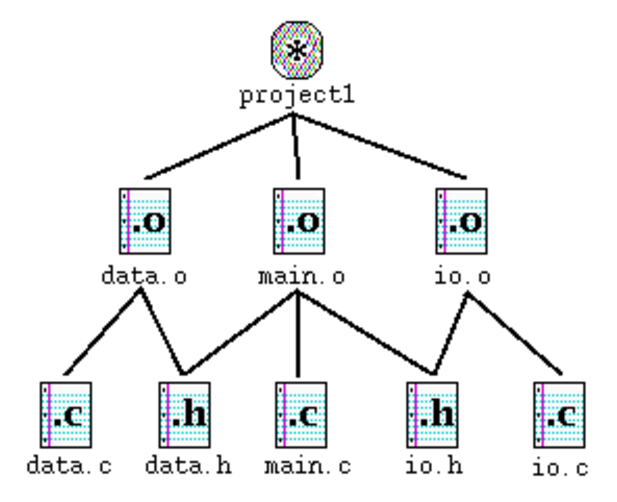
\includegraphics[height=4cm]{figures/depgraph.eps}
\caption{File dependencies in a project}
\label{default}
\end{center}
\end{figure}
\begin{figure}[htbp]
\begin{center}
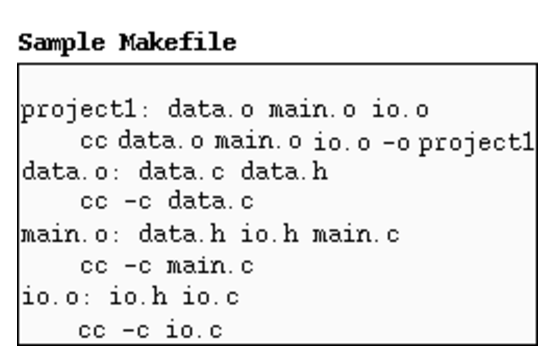
\includegraphics[height=4cm]{figures/makefile.eps}
\caption{The makefile}
\label{default}
\end{center}
\end{figure}
The makefile is made up of the following format:
\begin{verbatim}
target: source file(s)
		       command (note that the tab is required)
\end{verbatim}
and must be named {\bf makefile} or {\bf Makefile} if you wish to use the command ``make''. However it is possible to use a different makefile name by running the following command
\begin{verbatim}
make -f mymakefile
\end{verbatim}

\subsection{My simple makefile test}

I tried my own makefile to see if I could get things working and compile things much faster. I wrote a simple program in C++ contained in one file called 
\begin{verbatim}
mapTester.cpp
\end{verbatim}
I created a makefile as follows:
\begin{verbatim}
CC=g++
CFLAGS=-Wall

mapTester: mapTester.o

clean:
        rm -f mapTester mapTester.o
\end{verbatim}
And voila! When I type 'make' I create a compiled program (if I have changed anything in the source file) and when I type 'make clean' I remove the exectuble and the object file. Brilliant.


%\section{Macros in make}
%We can also use macros to define a set of files. And, since the make command knows that in order to create an object file it must use cc -c on the associated .c file, we can omit these files from the makefile. eg.
%\begin{verbatim}
%OBJECTS = data.o main.o io.o
%project1: $(OBJECTS)
%       cc $(OBJECTS) -o project1
%data.o: data.h
%main.o: data.h io.h
%io.o: io.h
%\end{verbatim}

\section{A more general makefile}

The previous section illustrated a very simple makefile, but in most cases we will end up with a much more complicated scenario where several source files and header files must be compiled and then linked together to produce the desired executable. To do this, Make allows us to make use of certain implicit rules that simplify the creation of a makefile. 

Say we have four source files main.cpp, car.cpp, vehicle.cpp and truck.cpp and three header files car.h, vehicle.h and truck.h.  If we were to compile everything separately, we would find that there would be four object files: main.o, car.o, vehicle.o and truck.o and these are linked together to produce the resulting executable. But Make allows us to compile and link very easily using the following file:
\begin{verbatim}
CC = g++
CFLAGS = -Wall

OBJECTS = main.o vehicle.o car.o truck.o

app : $(OBJECTS)
       $(CC) -o app $(OBJECTS)

main.o : vehicle.h car.h truck.h
vehicle.o : vehicle.h
car.o : car.h
truck.o : truck.h

clean:
       rm app $(OBJECTS)
\end{verbatim}

What might seem strange are the lines which list the dependencies for each of the object files. For example, the line 
\begin{verbatim}
main.o : vehicle.h car.h truck.h
\end{verbatim}
would usually be written as
\begin{verbatim}
main.o : main.cpp vehicle.h car.h truck.h
       $(CC) -c main.cpp 
\end{verbatim}
The reason we can write the latter is because Make has an implicit rule which says that every object file is compiled from a corresponding source file with the same name. And when we write
\begin{verbatim}
main.o : vehicle.h car.h truck.h
\end{verbatim}
it is implicitly assumed that the object is created using
\begin{verbatim}
$(CC) -c 
\end{verbatim}
with the same name as the object file.

\section{CMake}
\label{sec:cmake}

CMake is one of the most important developments for the task of
compiling programs on a variety of platforms. It allows us to worry
less about compiling the code on various machines since it has the
ability to create automatically Xcode project files (for the Mac),
Visual Studio files (for windows) and makefiles (for Linux). The idea
is that all the instructions for compiling and linking are given in a
file called CMakeLists.txt. To demonstrate the process, consider the
following directory structure that we might see in a project:
\begin{verbatim}
src/
include/
main.cpp
CMakeLists.txt
\end{verbatim}
The source files (eg. .cpp files) are kept in /src and header files
are kept in /include (e.g. .h files). The reason for this is to make
life easier if we distribute our code as a library where we must give
our header files alongside the libraries. The main.cpp is the usual
main entry point to our program.

The really interesting part though is the CMakeLists.txt file which
basically replaces the need to manually create a Makefile. In this
project our CMakeLists.txt file might look something like this
\begin{verbatim}
CMAKE_MINIMUM_REQUIRED( VERSION 2.6 )
PROJECT( cmaketest )

# the directory to look for header files
INCLUDE_DIRECTORIES( include )

# using a 'globbing' approach where we find all the .cpp files and make them our source files
FILE( GLOB SOURCES src/*.cpp )
MESSAGE( "SOURCES = " ${SOURCES} )

# define the library path
SET(LIBRARY_OUTPUT_PATH ${cmaketest_BINARY_DIR}/lib)

# create a library
ADD_LIBRARY( mylib ${SOURCES} )

# create an executable
ADD_EXECUTABLE( cmakeTestExec main.cpp )
TARGET_LINK_LIBRARIES( cmakeTestExec mylib )
\end{verbatim}

Let's go through this line by line.

\begin{enumerate}
\item First, we must tell cmake the minimum version of cmake that is
  required. 2.6 seems to be quite common at the moment.
\item Define the project name that will be used in later commands.
\item Tell the compiler where to look for header files when compiling
  (ie. the -I flag).
\item Define a variable called SOURCES which is made up of all the
  source files for our project. In this case we look in the src/
  directory for all files ending in .cpp.
\item Display a message which lists all the source files (as a check
  for the user of cmake).
\item The default library path is the same as the build directory, but
  in this case we have decided to include the libraries in a folder
  called 'lib'. This will be seen in the build directory.
\item We create a library called mylib by compiling the source files.
\item We create an executable from main.cpp.
\item We must link the previously created executable with the library
  we have just created.
\end{enumerate}

\subsection{Using ccmake}
\label{sec:using-ccmake}


What we have done in the previous section is set up the rules that
will allow us to create a ``build'' of the project. That is, we can
create a folder that will contain the executable and library files for
the project after compilation on our machine. Since different
computers have different ``architectures'' we may need to create
several builds for each different type.

Let's assume we are in the directory of the source code which contains
the file main.cpp\footnote{Look in ~/Documents/programming/cmake/cmakeDemo to find these files on my computer}. We can create a build directory here by 
\begin{verbatim}
mkdir build
\end{verbatim}
We can change into this directory with
\begin{verbatim}
cd build/
\end{verbatim}
We can now run ccmake, which is a GUI for cmake as follows:
\begin{verbatim}
ccmake ../
\end{verbatim}
This tell ccmake to look in the directory above for the CMakeLists.txt
file. You will see a table of values which have been automatically
created by CMake. In some cases we might need to change these, like in
the case when we specify the location of a library. But for this
simple project we can simply type
\begin{verbatim}
c
\end{verbatim}
which will show a message of all the source files. We exit this by
typing
\begin{verbatim}
e
\end{verbatim}
We can then generate the makefile by typing
\begin{verbatim}
g
\end{verbatim}
You should now see a makefile in the current directory. This allows us
to compile the code to produce the executable and the library by
simply typing
\begin{verbatim}
make
\end{verbatim}

Essentially, we have greatly simplified the creation of makefiles
which can often be problematic for cross-platform compiling (ie
producing libraries and executables on different machines).

%%% Local Variables: 
%%% mode: latex
%%% TeX-master: "Programming"
%%% End: 


\part{Frameworks and libraries}
\chapter{Accelerate framework}

\section{ARM architecture/NEON}

\subsection{ARMv7}
\begin{itemize}
\item Used in iphone 3Gs, ipad, iphone 4, ipod 3rd generation touch. 
\item SIMD unit called NEON
\item eg. the function 
\begin{verbatim}
vmul.f32 qo, q1, q2
\end{verbatim}
will multiply four 32-bit floats from q2 with four 32-bit floats from q1 and store the result in q0.
\item The point is that this is done {\bf simulataneously}.
\item NEON does not use double precision units.
\item NEON may use more power but, since the instructions will take less time, overall they may be more efficient.
\end{itemize}

\section{What can be done in the accelerate framework}

\begin{itemize}
\item New to iphone 4.0.
\item Consists of many libraries, only three of which are currently available in iphone os 4.0. These are vDSP, LAPACK and BLAS.
\item vDSP (Digital Signal Processing library). 
\item eg. Dot product
\begin{verbatim}
#include <Accelerate/Accelerate.h>

float dotProduct;
vDSP_dotpr(a, 1, b, 1, &dotProduct, n);  // take in pointers to two arrays 
\end{verbatim}
\item This code is 8x faster than simple for loop. We also use approx. 1/4 of the energy.
\item Important to note that this can be used on different hardware.
\end{itemize}

\subsection{LAPACK}
\begin{itemize}
\item Been around a long time.
\item High level linear algebra.
\item Matrix factorisations.
\item Eigenvalues/vectors
\item Single/Double precision
\item Real/complex data types
\item Different matrix types
\item Because it comes from Fortran, it is laid out in column major order
\begin{verbatim}
float b[n];
b[0]=5.f; b[1]  = 5.f; b[2] = 4.f; b[3] = -2.f;

__CLPK_integer nrhs = 1;
__CLPK_integer ipiv[n];
__CLPK_integer info;

sgesv_(&n, &nrhs, A, &n, ipiv, b, &n, &info);
printf(``The solution is: (\%f, \%f, \%f, \%f)\n'', b[0],b[1], b[2], b[3]);

\end{verbatim}
\item when we compile this we must link against the accelerate framework eg.
\begin{verbatim}
gcc lapack.c -framework Accelerate -std=c99 -o lapackExample
./lapackExample
\end{verbatim}
\item The -std=c99 flag specifies we are using the 1999 standard of C.
\end{itemize}

\subsection{BLAS}

\begin{itemize}
\item Low level stuff
\item eg. Dot product, vector products
\item Matrix-vector products
\item Matrix multiplies
\item Supports for both row and column major order
\item Can use dense and triangular matrices
\begin{verbatim}
#include <Accelerate/Accelerate.h>
#include <stdio.h>
int main()
{
float A[2][2] = {{1.f, 1.f}, 
		        {0.f, 1.f}};
float B[2][2] = {{1.f, 2.f}, 
		        {3.f, 4.f}};	
float C[2][2];

cblas_sgemm(CblasRowMajor, CblasNoTrans, CblasNoTrans,
    		    2, 2, 2, 1.f, A, 2, B, 2, 0.f, C, 2);	
     		    
printf("%f, %f, %f, %f\n", C[0][0], C[0][1], C[1][2], C[2][2]);

return(0);
}        	        	
\end{verbatim}
\end{itemize}












\chapter{Diffpack framework}

This is a project that I have started to get involved with since March 2011 and has the potential to be quite fruitful. Diffpack is a numerical analysis software library that allows a huge variety of problems to be solved using various numerical methods. There are finite difference and finite element implementations that are capable of solving various linear and non-linear problems and there are variety of solvers available to the user. However, on a first introduction to the software, it may seem quite daunting to use, especially if the user's programming background is limited. Therefore, there are a few points to bear in mind when learning about Diffpack
\begin{itemize}
\item  You will still have to program in C++! The idea with Diffpack is that you write software that will use the various libraries containing all the magical numerical code but there are certain functions that you will need to write to get something to work.
\item Diffpack only really deals with the analysis stage in the solution procedure. It assumes that a mesh has already been created (Diffpack has some limited meshing capabilities) at the start and once the problem has been solved, it will output the result to certain files (output files). If the user wants to visualise the results in some nice graphical format, then it is possible to use various scripts that will convert it to formats like .VTK which allow it to visualised in programs like Paraview. 
\item You will spending most of your time at the terminal screen! There is a GUI that can be used, but you will mostly be compiling and using the code through the terminal. This may take some getting used to! Some techniques which should be practised include: compiling code, changing directories,  moving directories, executing code.
\end{itemize}

\section{Installation on Ubuntu}
Now this is a task and a half (well so it felt at the time). There are a few things that were not immediately obvious to me during the process. Here are some pointers
\begin{enumerate}
\item The first thing to do is to copy the files from the cd to an appropriate directory. In all the examples given by Diffpack, it is installed in /usr/local/, so I just put the files there.
\item I created a temporary folder called dptmp and within this I put the folder kernel (of the appropriate architecture type). eg. for a 32-bit linux system this folder is in the linux-gcc402 folder on the cd.
\item We then issue the following command to run the installation script 
\begin{verbatim}
sh dptmp/kernel/install-dp.sh -r /usr/local -m linux-gcc-4.0.2 
-s /usr/local/dptmp/kernel
\end{verbatim}
\item We now need to edit the .profile file by placing come lines at the end. We can edit it by typing {\bf sudo vi ~/.profile}. We then put the following lines at the end of the file
\begin{verbatim}
export NOR=/usr/local/NO
export MACHINE_TYPE=linux-gcc-4.0.2
. $NOR/etc/setup/dpshrc
\end{verbatim} 
\item We are now able to create a project with Diffpack by changing to a suitable directory and then issuing the command {\bf Mkdir newprojectname}. This will create a folder where we will store our source files. 
\item We can create a file called {\bf newprojectname.cpp} and in this we can use all the various Diffpack classes and variable types to get a FE code running. Once we have saved the file we can compile and link the code just by simply typing {\bf Make}.
\item However, on my first attempt it didn't compile straight away since there were several libraries that I needed to install. For example, I got the error about some library called -lXext - this is solved by going into the Ubuntu package manager, searching for the library and installing it. This may have to be done for several libraries\footnote{Some of the packages I needed to install were Xext, libxt6-dbg, libxt-dev, x11proto-xext-dev, tcl, osmesa, tk8}.
\item Finally, it is necessary to get a licence key for Diffpack which requires both a hostname and hostid. We can get the hostname by typing {\bf uname -a}. But to get the hostid I need to change into the directory \$NOR/ext/FLEXlm/linux-gcc-4.0.2 and run the command {\bf ./lmutil lmhostid}
\end{enumerate}

\section{Installation on Mac OS X}

Installation on a Mac is also possible, although it is clear that it is not supported by the team in Nurnburg. We follow much the same process as for linux, making sure that we change the MACHINE TYPE and copy the correct diffpack kernel into our installation directory. Once we have things installed, there were a few things that were a bit unusual:
\begin{itemize}
\item I edited my .bashrc file (this is kept in the home folder\footnote{we get here by typing cd $\sim$}) and it looks like
\begin{verbatim}
export PATH=.:$PATH
export NOR=/usr/local/Diffpack/NO/
export MACHINE_TYPE=mac-gcc-4.2
. /usr/local/Diffpack/NO/etc/setup/dpshrc
\end{verbatim}
\item It appears the the commands Mkdir and Make which are Diffpack specific do not work in mac directly since we find that the commands are case-insensitive in mac (ie. Mkdir is the same as mkdir). So to run the specific Diffpack commands we would need to type, for example
\begin{verbatim}
$NOR/bin/Mkdir
\end{verbatim}
\item We can also use Diffpack through Xcode which makes debugging a lot easier. There is a pdf created by the people at diffpack explaining these details, but it is probably easier just to email me\footnote{robertnsimpson@gmail.com} since I can send you a working xcode project with all the Diffpack settings.
\end{itemize}















\part{Parallel programming}
\chapter{Merlin (Cardiff)}

\section{Preliminaries}

\subsection{Logging in}


Fire up a terminal and type in 
\begin{verbatim}
ssh -X <username> merlinlogin01.arcca.cf.ac.uk
\end{verbatim}

\subsection{Compiling a simple project}

Load the modules
\begin{verbatim}
module load intel/compilers/11
module load intel/mpi/4.0
\end{verbatim}

and compile with mpi
\begin{verbatim}
mpicc -o app hello.c
\end{verbatim}

And submit the job with an appropriate qsub script
\begin{verbatim}
qsub batch.pbs
\end{verbatim}

Appropriate output files will be created.






\appendix

\chapter{Notes on C}
\label{cha:appendix}

\section{size\textunderscore t}
\label{sec:size_t}

The type \verb=size_t= is used as the return type for the
\verb=sizeof= function in C. We might use it in the following way
\begin{lstlisting}
int n = 10;
size_t size = sizeof(int) * n;
int* p = malloc( size_t );
\end{lstlisting}


%%% Local Variables: 
%%% mode: latex
%%% TeX-master: "Programming"
%%% End: 

\end{document}